% ============================================================
%  MÓDULO 23 — Atlas de infográficos NotebookLM (R101)
%  6 PNGs curtos revisados, textos curtos, ortografia conferida
% ============================================================
\chapter{Atlas Visual: Seis Infográficos do NotebookLM}

\roteirodidatico
{Seis imagens valem mais que sessenta parágrafos quando mostram o mesmo caminho com ícones. Este atlas reúne os infográficos gerados no caderno Livro Core Infográficos Didáticos R100, versão curta revisada (R101): textos curtos, ortografia conferida, cada figura com fonte e capítulo.}
{\emph{Infográfico} resume visualmente um capítulo; \emph{Atlas} é a coleção ordenada; \emph{Revisão humana} é a conferência do texto da imagem contra o capítulo.}
{Olhe a imagem, leia a legenda de uso e confira o capítulo indicado antes de citar a figura.}
{Imagem gerada por IA pode conter deslize de número em ícone; só o texto do capítulo e a fonte primária valem como prova.}
{Que figura você mostraria a alguém em 1 minuto para explicar o Core?}

\casoguiado{Bruno imprime, Ana aponta}
{Bruno imprime as seis em A4 e espalha na mesa. Ana aponta para a casa de 8 andares e pergunta onde mora o fiscal. Bruno aponta a camada da qualidade. Ela aponta a encomenda em 7 passos e pergunta onde fica a nota. Ele aponta o passo 3. Cada apontar termina com a mesma frase: agora confira no capítulo.}

\section{As seis figuras e onde usá-las}

\elemento{INF-S01 — A casa de 8 andares}{\metainfo{ID}{INF-S01} \hfill \metainfo{Arquivo}{\pth{INF-S01-casa-curta.png}} \hfill \metainfo{Capítulo}{mod-01d e mod-02}}

\begin{descricao}
Vista geral das camadas com ícones e frases curtas: fundação, entrada, maestro, qualidade e topo. Use para abrir qualquer explicação: comece pelo todo antes do detalhe.
\end{descricao}

\begin{center}
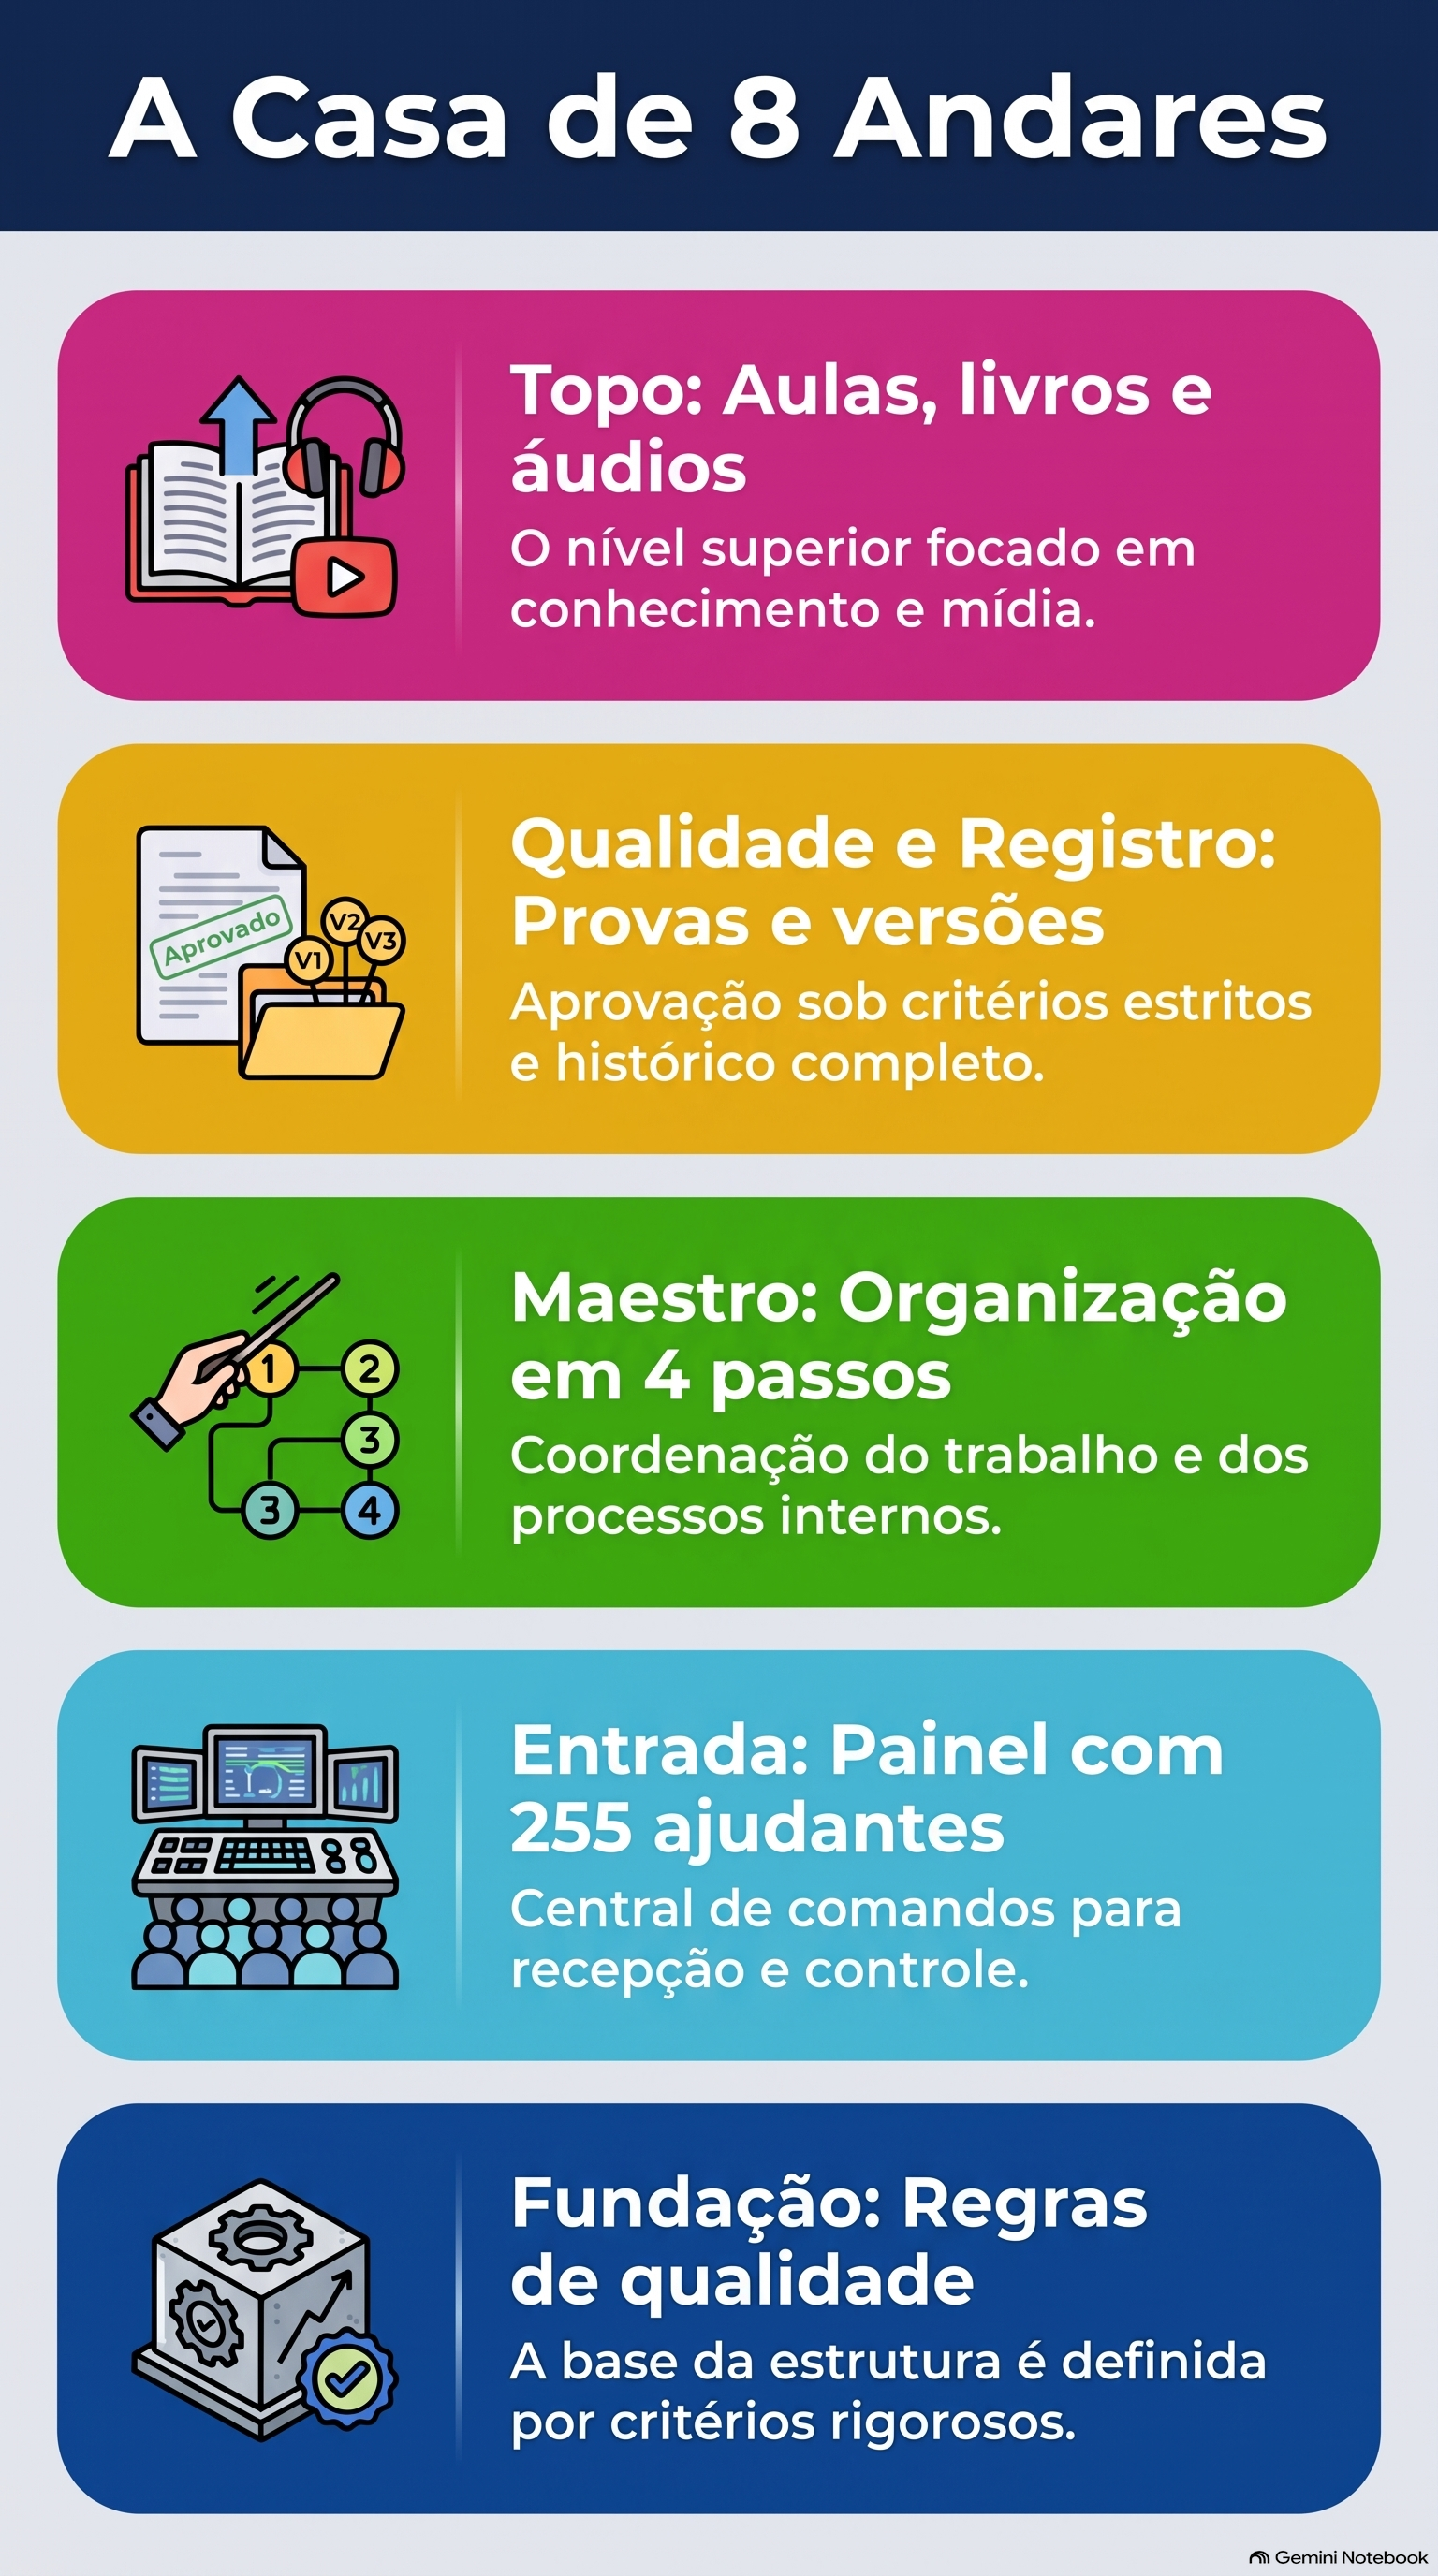
\includegraphics[width=0.96\linewidth,height=0.80\textheight,keepaspectratio]{INF-S01-casa-curta.png}
\end{center}

\begin{aviso}
Figura gerada por IA a partir de roteiro curto do autor (ortografia do texto principal conferida visualmente). Detalhes de ícone podem divergir; para citar, use os nomes do texto: \pth{marceloclaro/orchestrator.py}, \pth{opencode.json}, \pth{mci/}. Caderno: Livro Core Infográficos Didáticos R100, pasta \pth{output/infografico-R101}. A primeira versão longa (R100, com erros de rótulo) fica arquivada em \pth{output/infografico-R100} e não entra no livro.
\end{aviso}

\elemento{INF-S02 — Ciclo em 4 fases}{\metainfo{ID}{INF-S02} \hfill \metainfo{Arquivo}{\pth{INF-S02-ciclo-curto.png}} \hfill \metainfo{Capítulo}{mod-02}}

\begin{descricao}
O laço Percebe, Delega, Executa, Reflete com rastro mínimo (critério, prova, registro, memória). Use para responder como uma tarefa atravessa o Core sem pular verificação.
\end{descricao}

\begin{center}
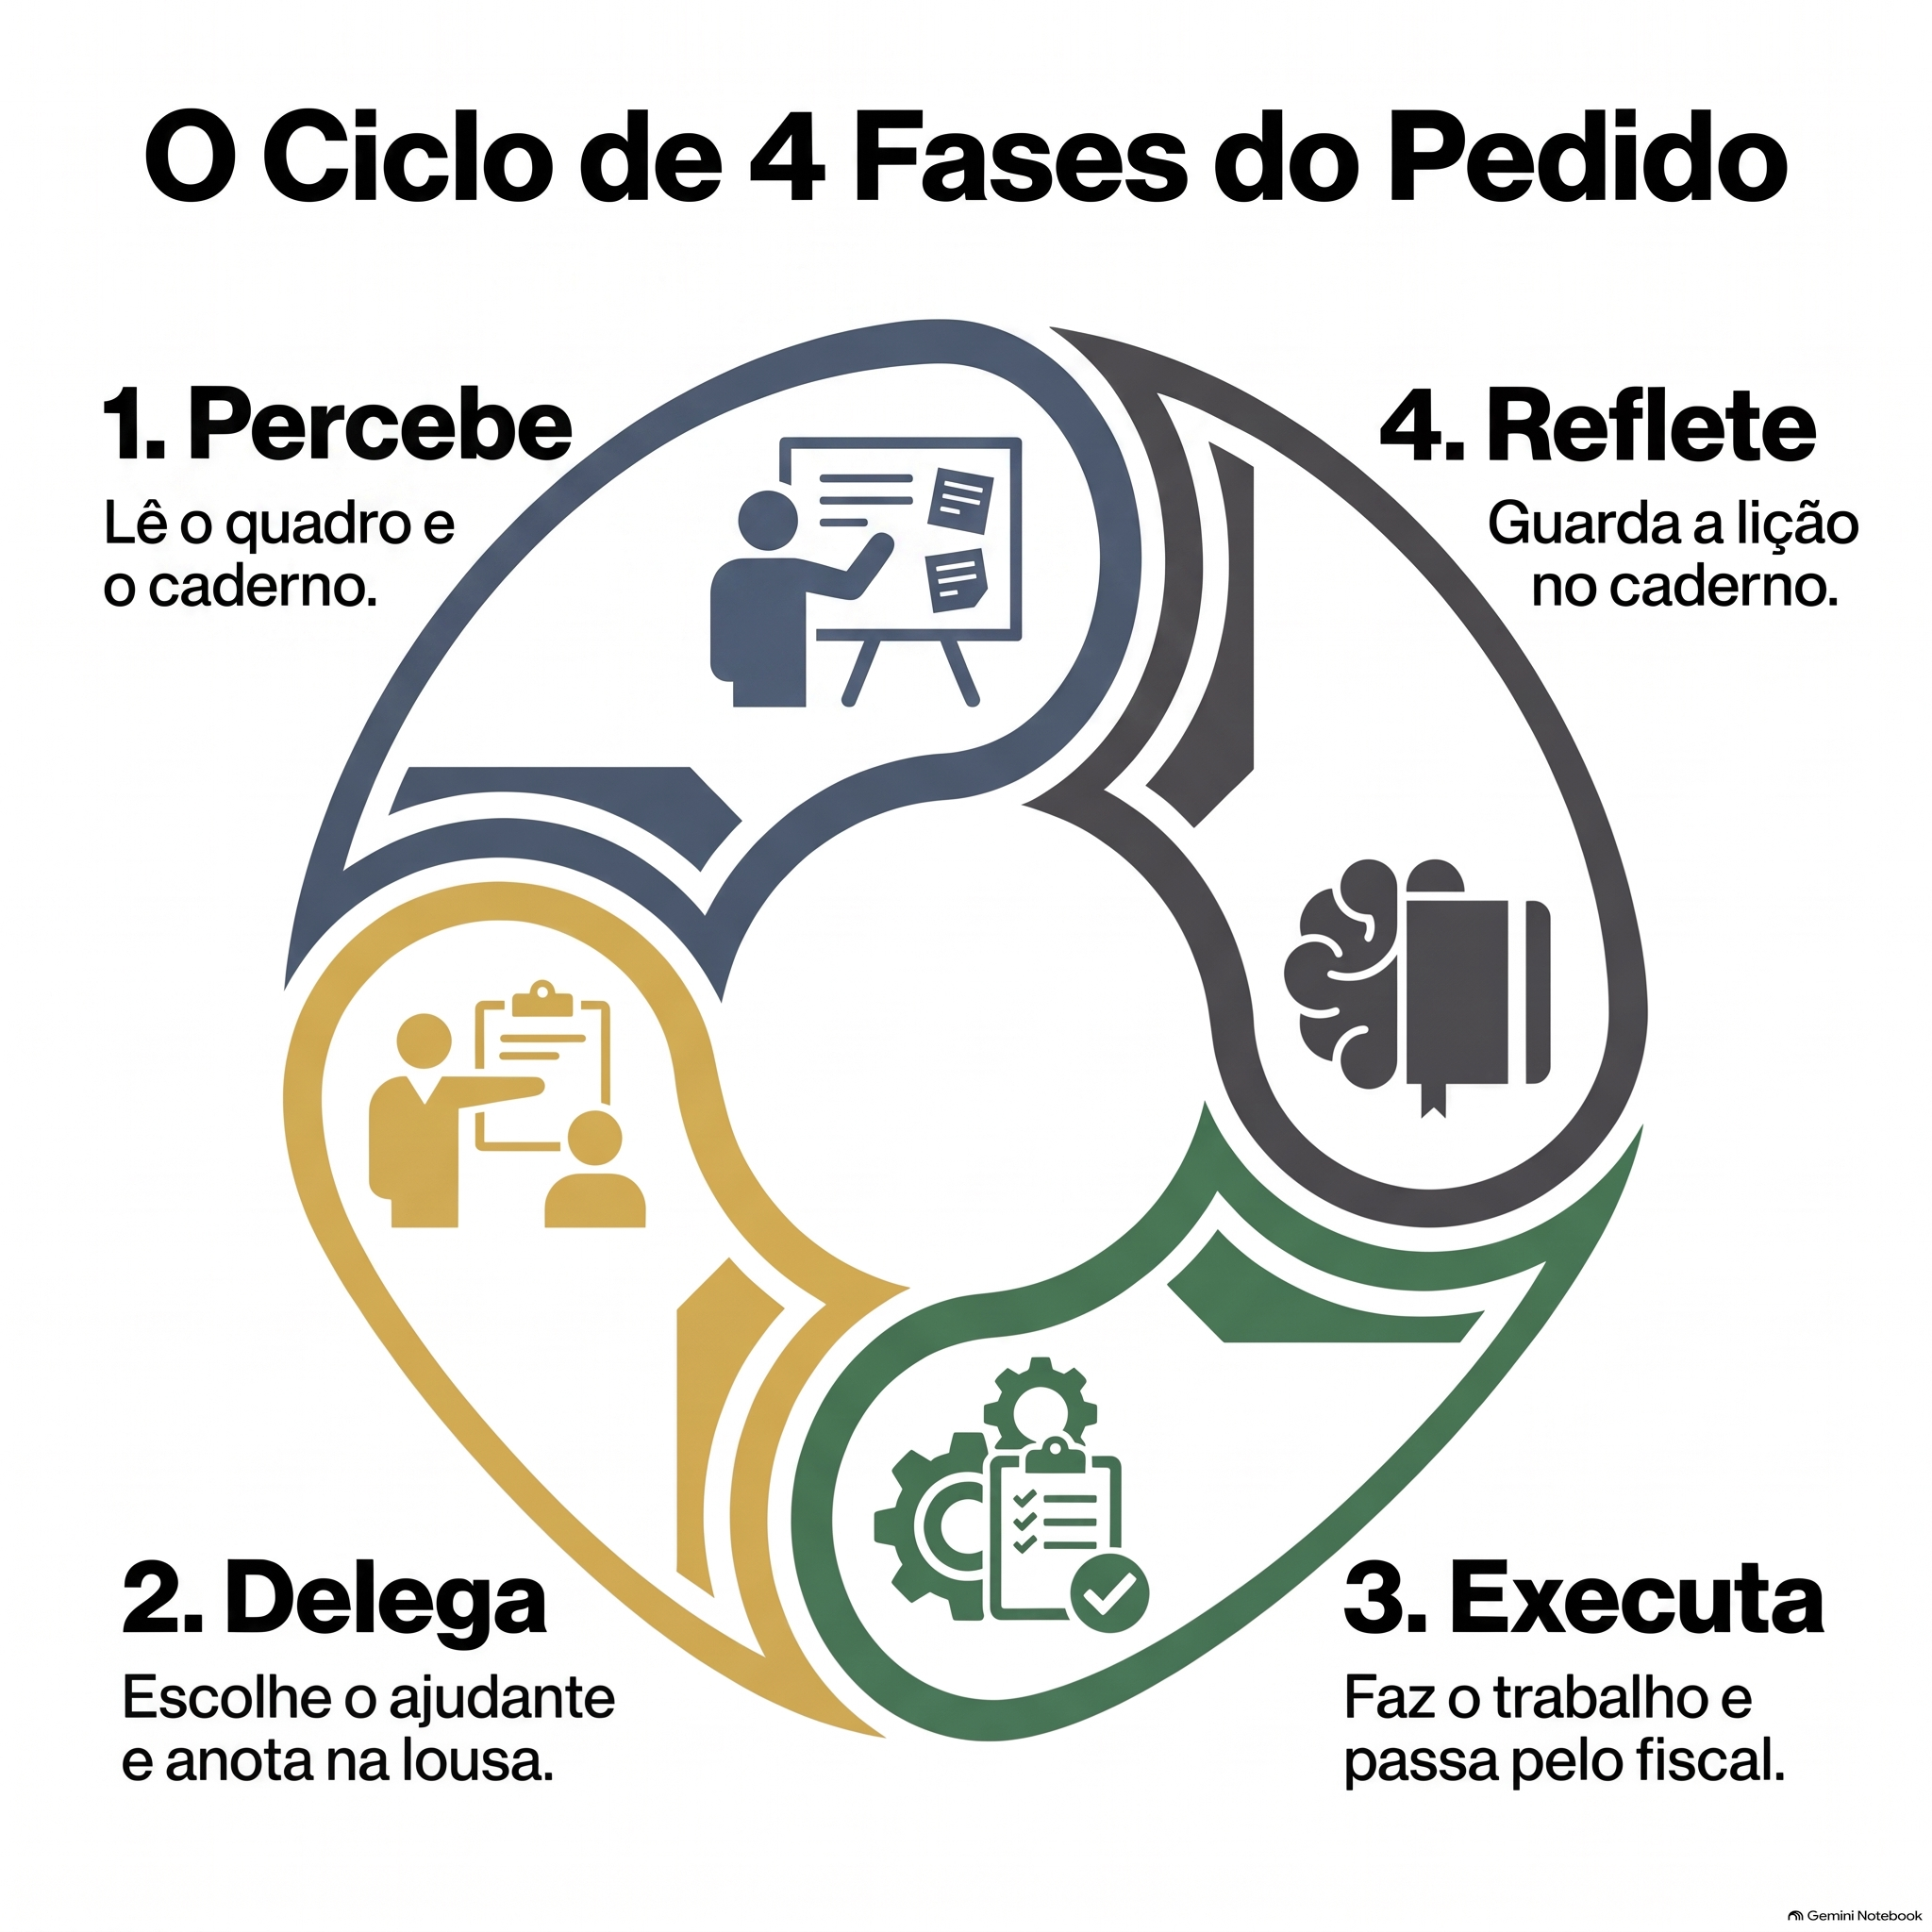
\includegraphics[width=0.96\linewidth,height=0.80\textheight,keepaspectratio]{INF-S02-ciclo-curto.png}
\end{center}

\elemento{INF-S03 — Encomenda em 7 passos}{\metainfo{ID}{INF-S03} \hfill \metainfo{Arquivo}{\pth{INF-S03-passos-curta.png}} \hfill \metainfo{Capítulo}{mod-17}}

\begin{descricao}
A encomenda de Ana em 7 passos numerados: balcão, placas, nota, lousa, oficina, fiscal e entrega com fonte. Use com leigos absolutos antes de qualquer código.
\end{descricao}

\begin{center}
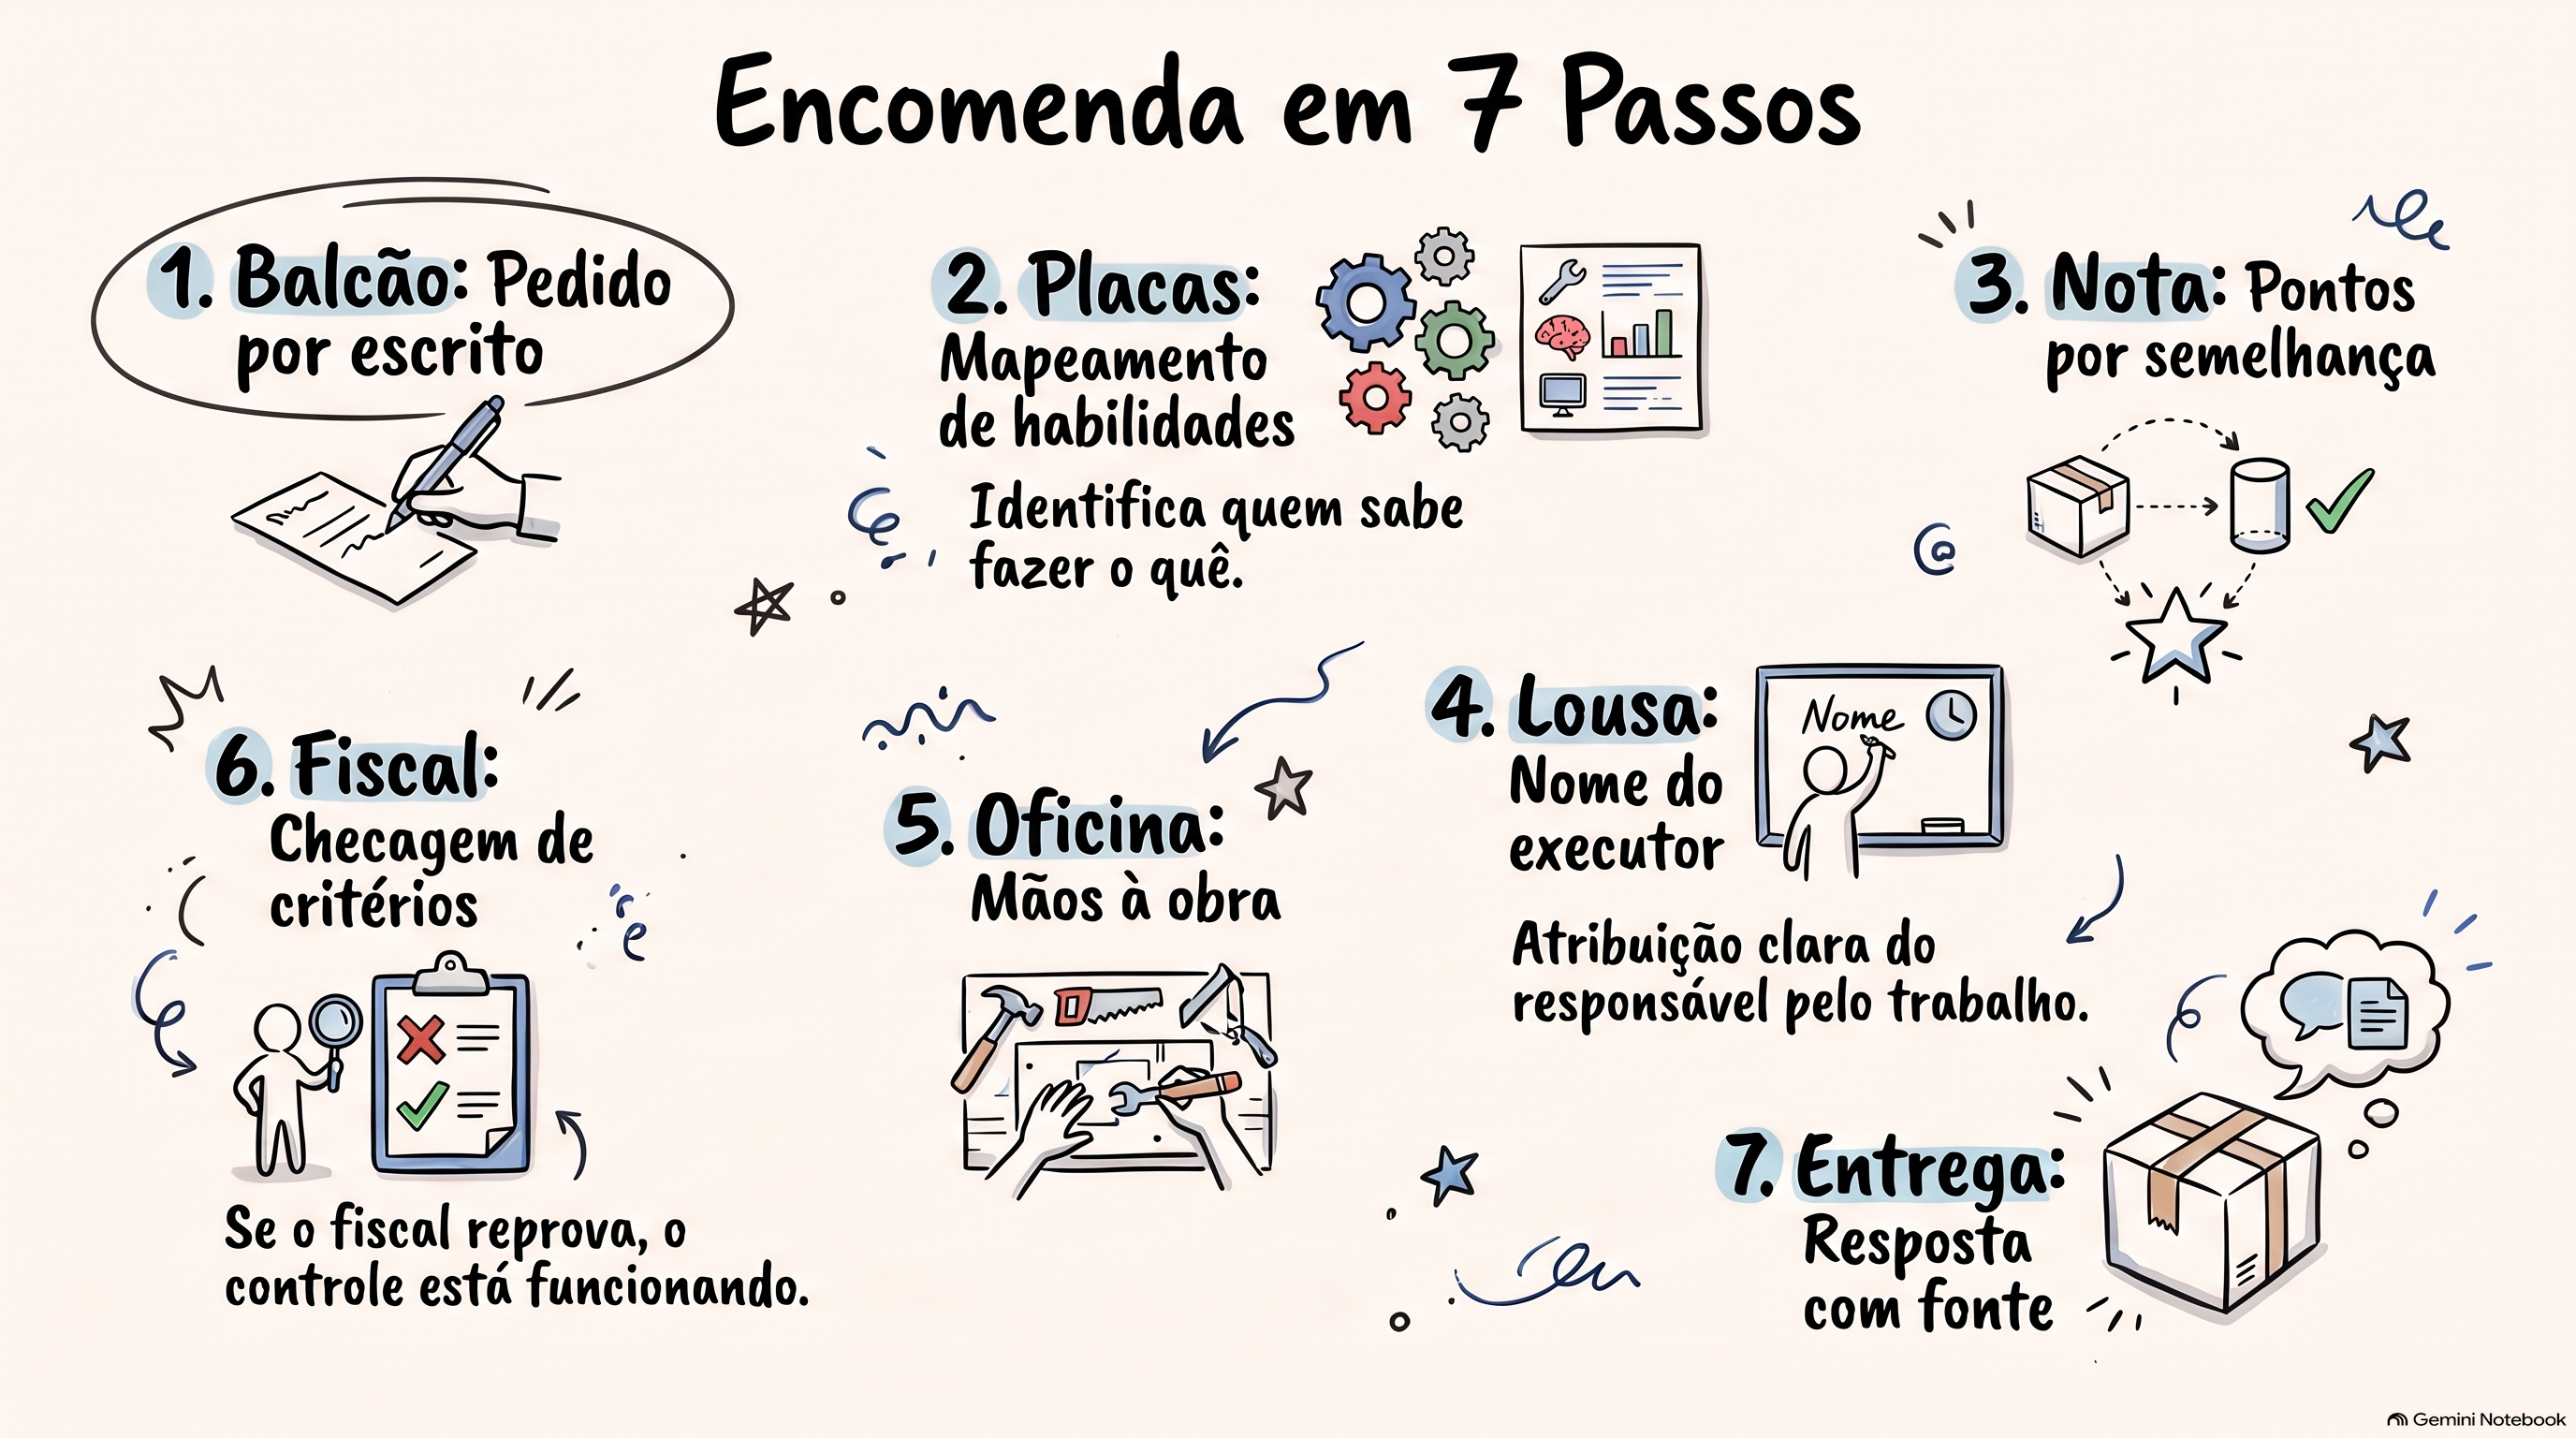
\includegraphics[width=0.96\linewidth,height=0.80\textheight,keepaspectratio]{INF-S03-passos-curta.png}
\end{center}

\elemento{INF-S04 — Lousa e caderno}{\metainfo{ID}{INF-S04} \hfill \metainfo{Arquivo}{\pth{INF-S04-lousa-curta.png}} \hfill \metainfo{Capítulo}{mod-03}}

\begin{descricao}
Quadro negro (trabalho: tarefas e voluntários) versus caderno (memória: histórico e lições). Use para fixar que trabalho é diferente de memória e que mensagem enviada não é tarefa pronta.
\end{descricao}

\begin{center}
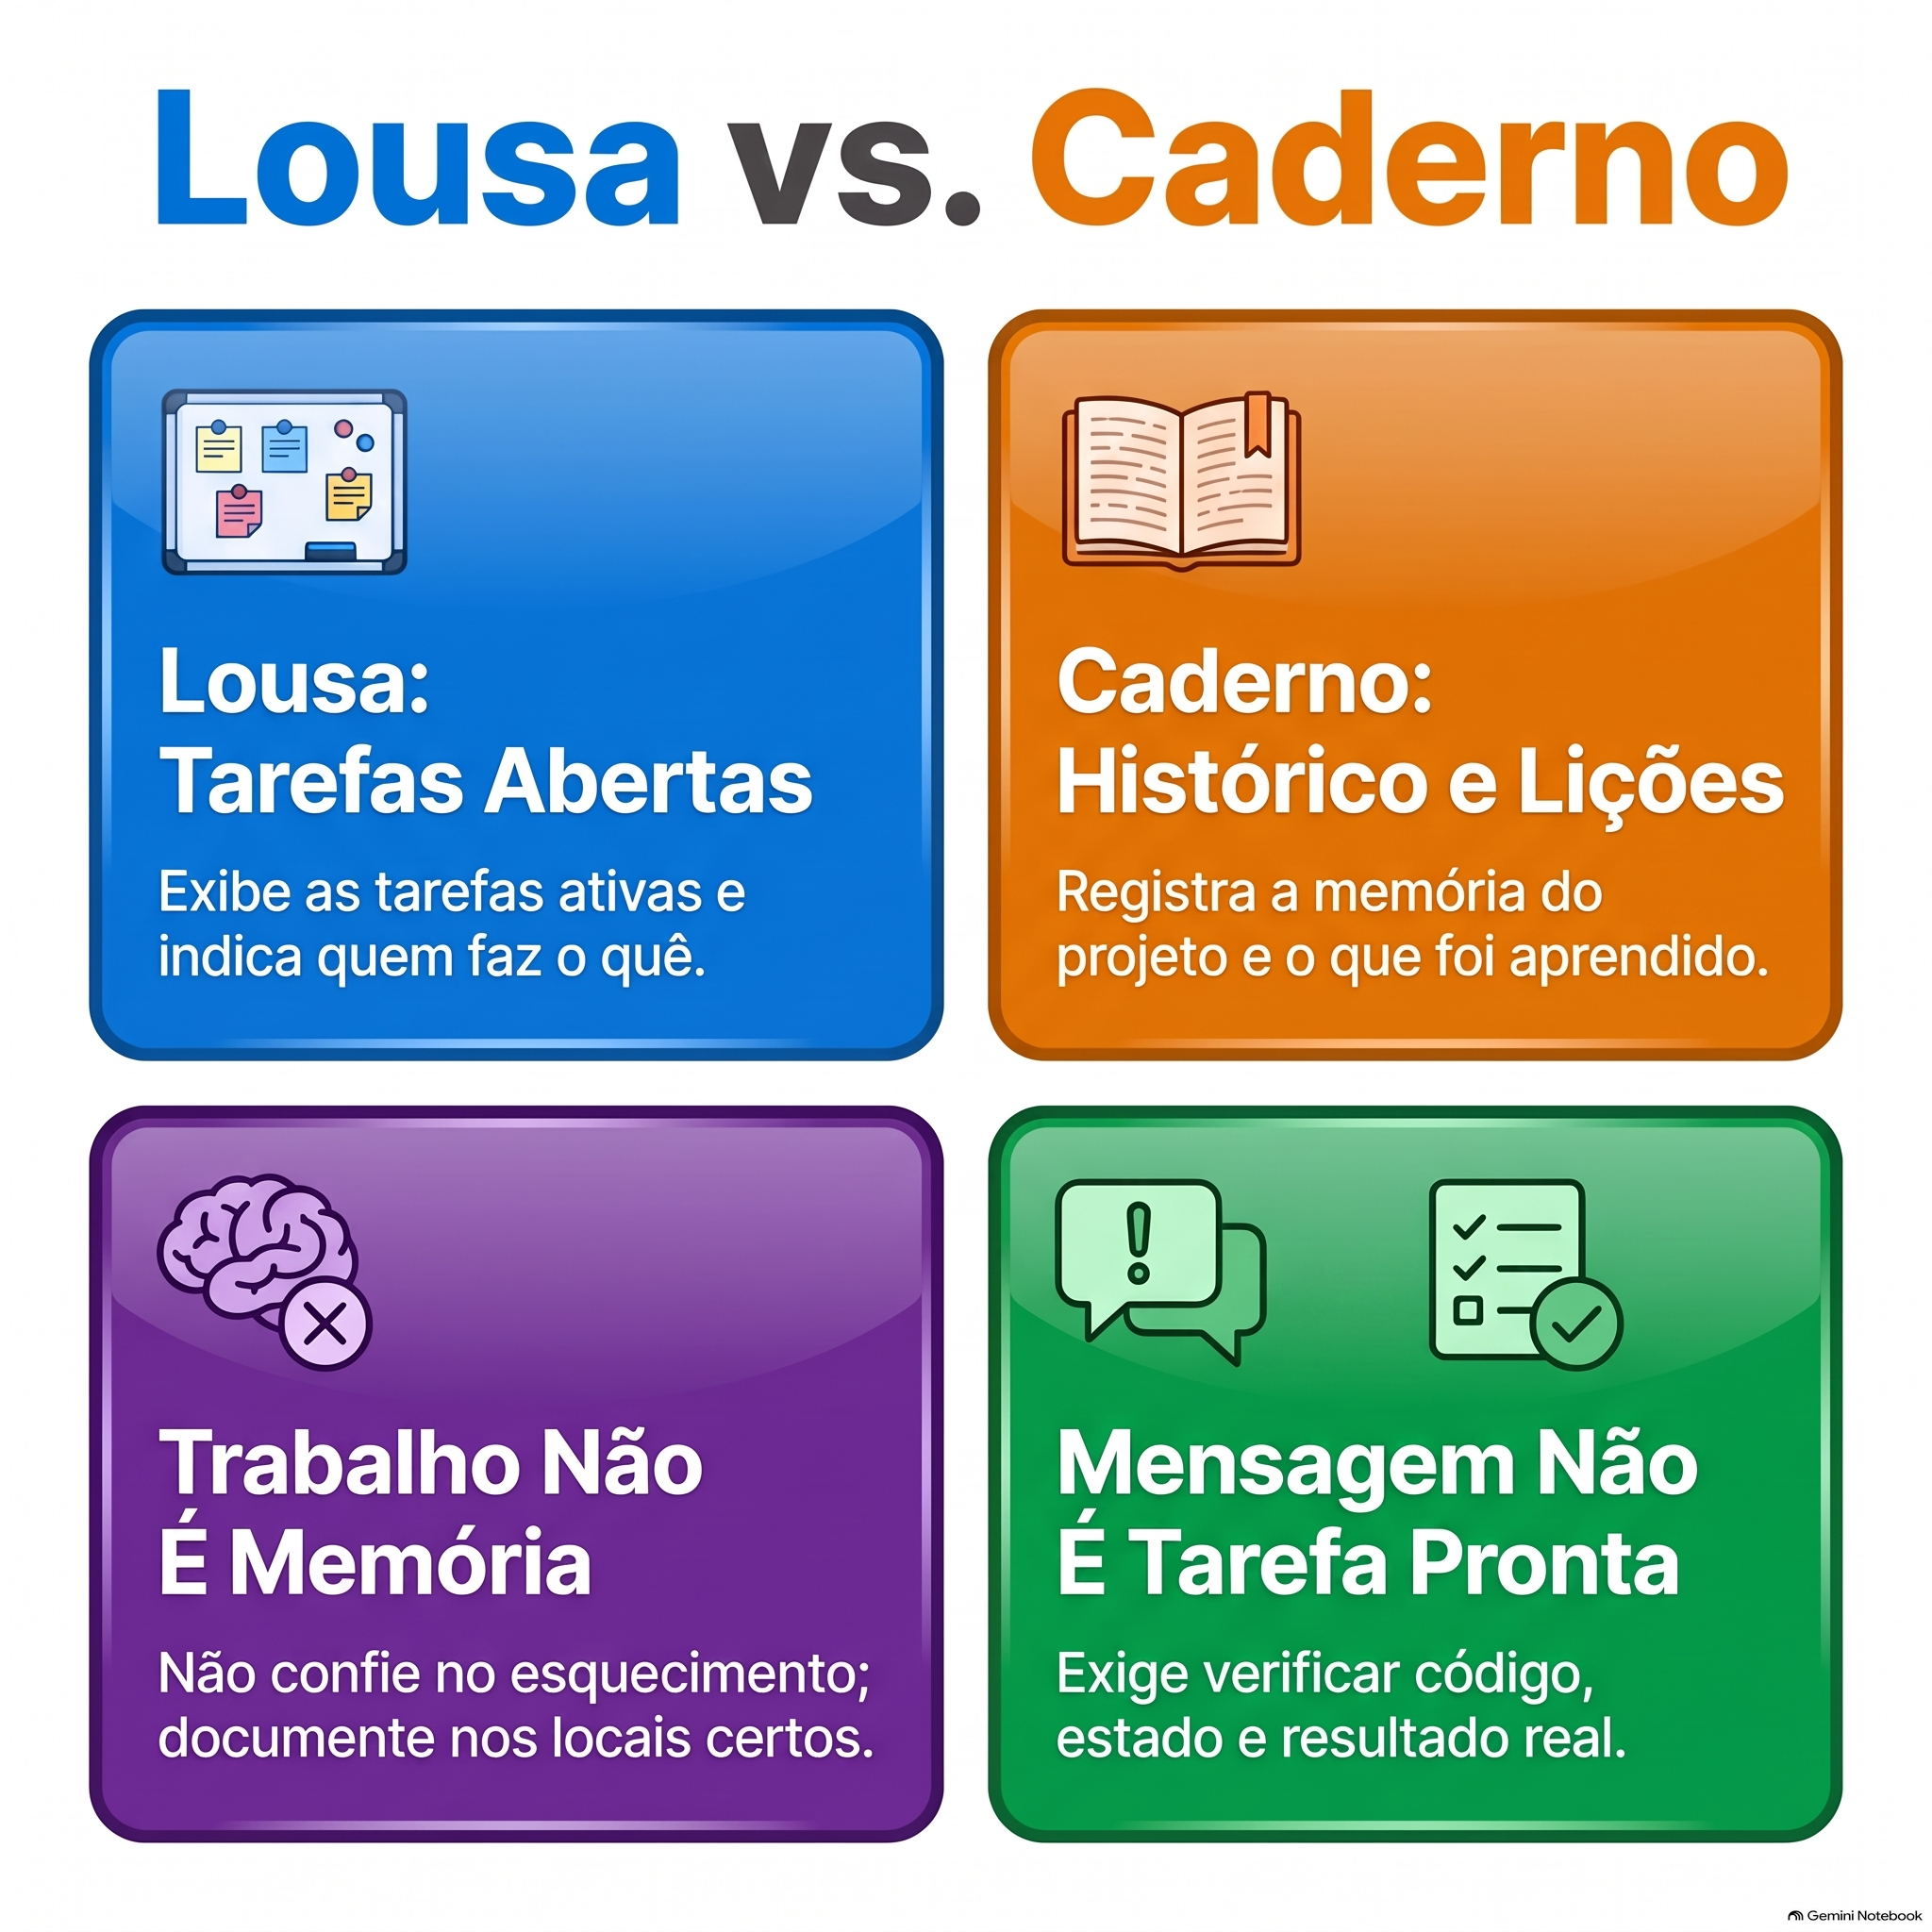
\includegraphics[width=0.96\linewidth,height=0.80\textheight,keepaspectratio]{INF-S04-lousa-curta.png}
\end{center}

\elemento{INF-S05 — Fiscal fechado}{\metainfo{ID}{INF-S05} \hfill \metainfo{Arquivo}{\pth{INF-S05-fiscal-curto.png}} \hfill \metainfo{Capítulo}{mod-04}}

\begin{descricao}
Combinado antes (regra escrita), prova depois (teste com gabarito) e fiscal que reprova na dúvida. Use para justificar por que prova verde não é selo geral.
\end{descricao}

\begin{center}
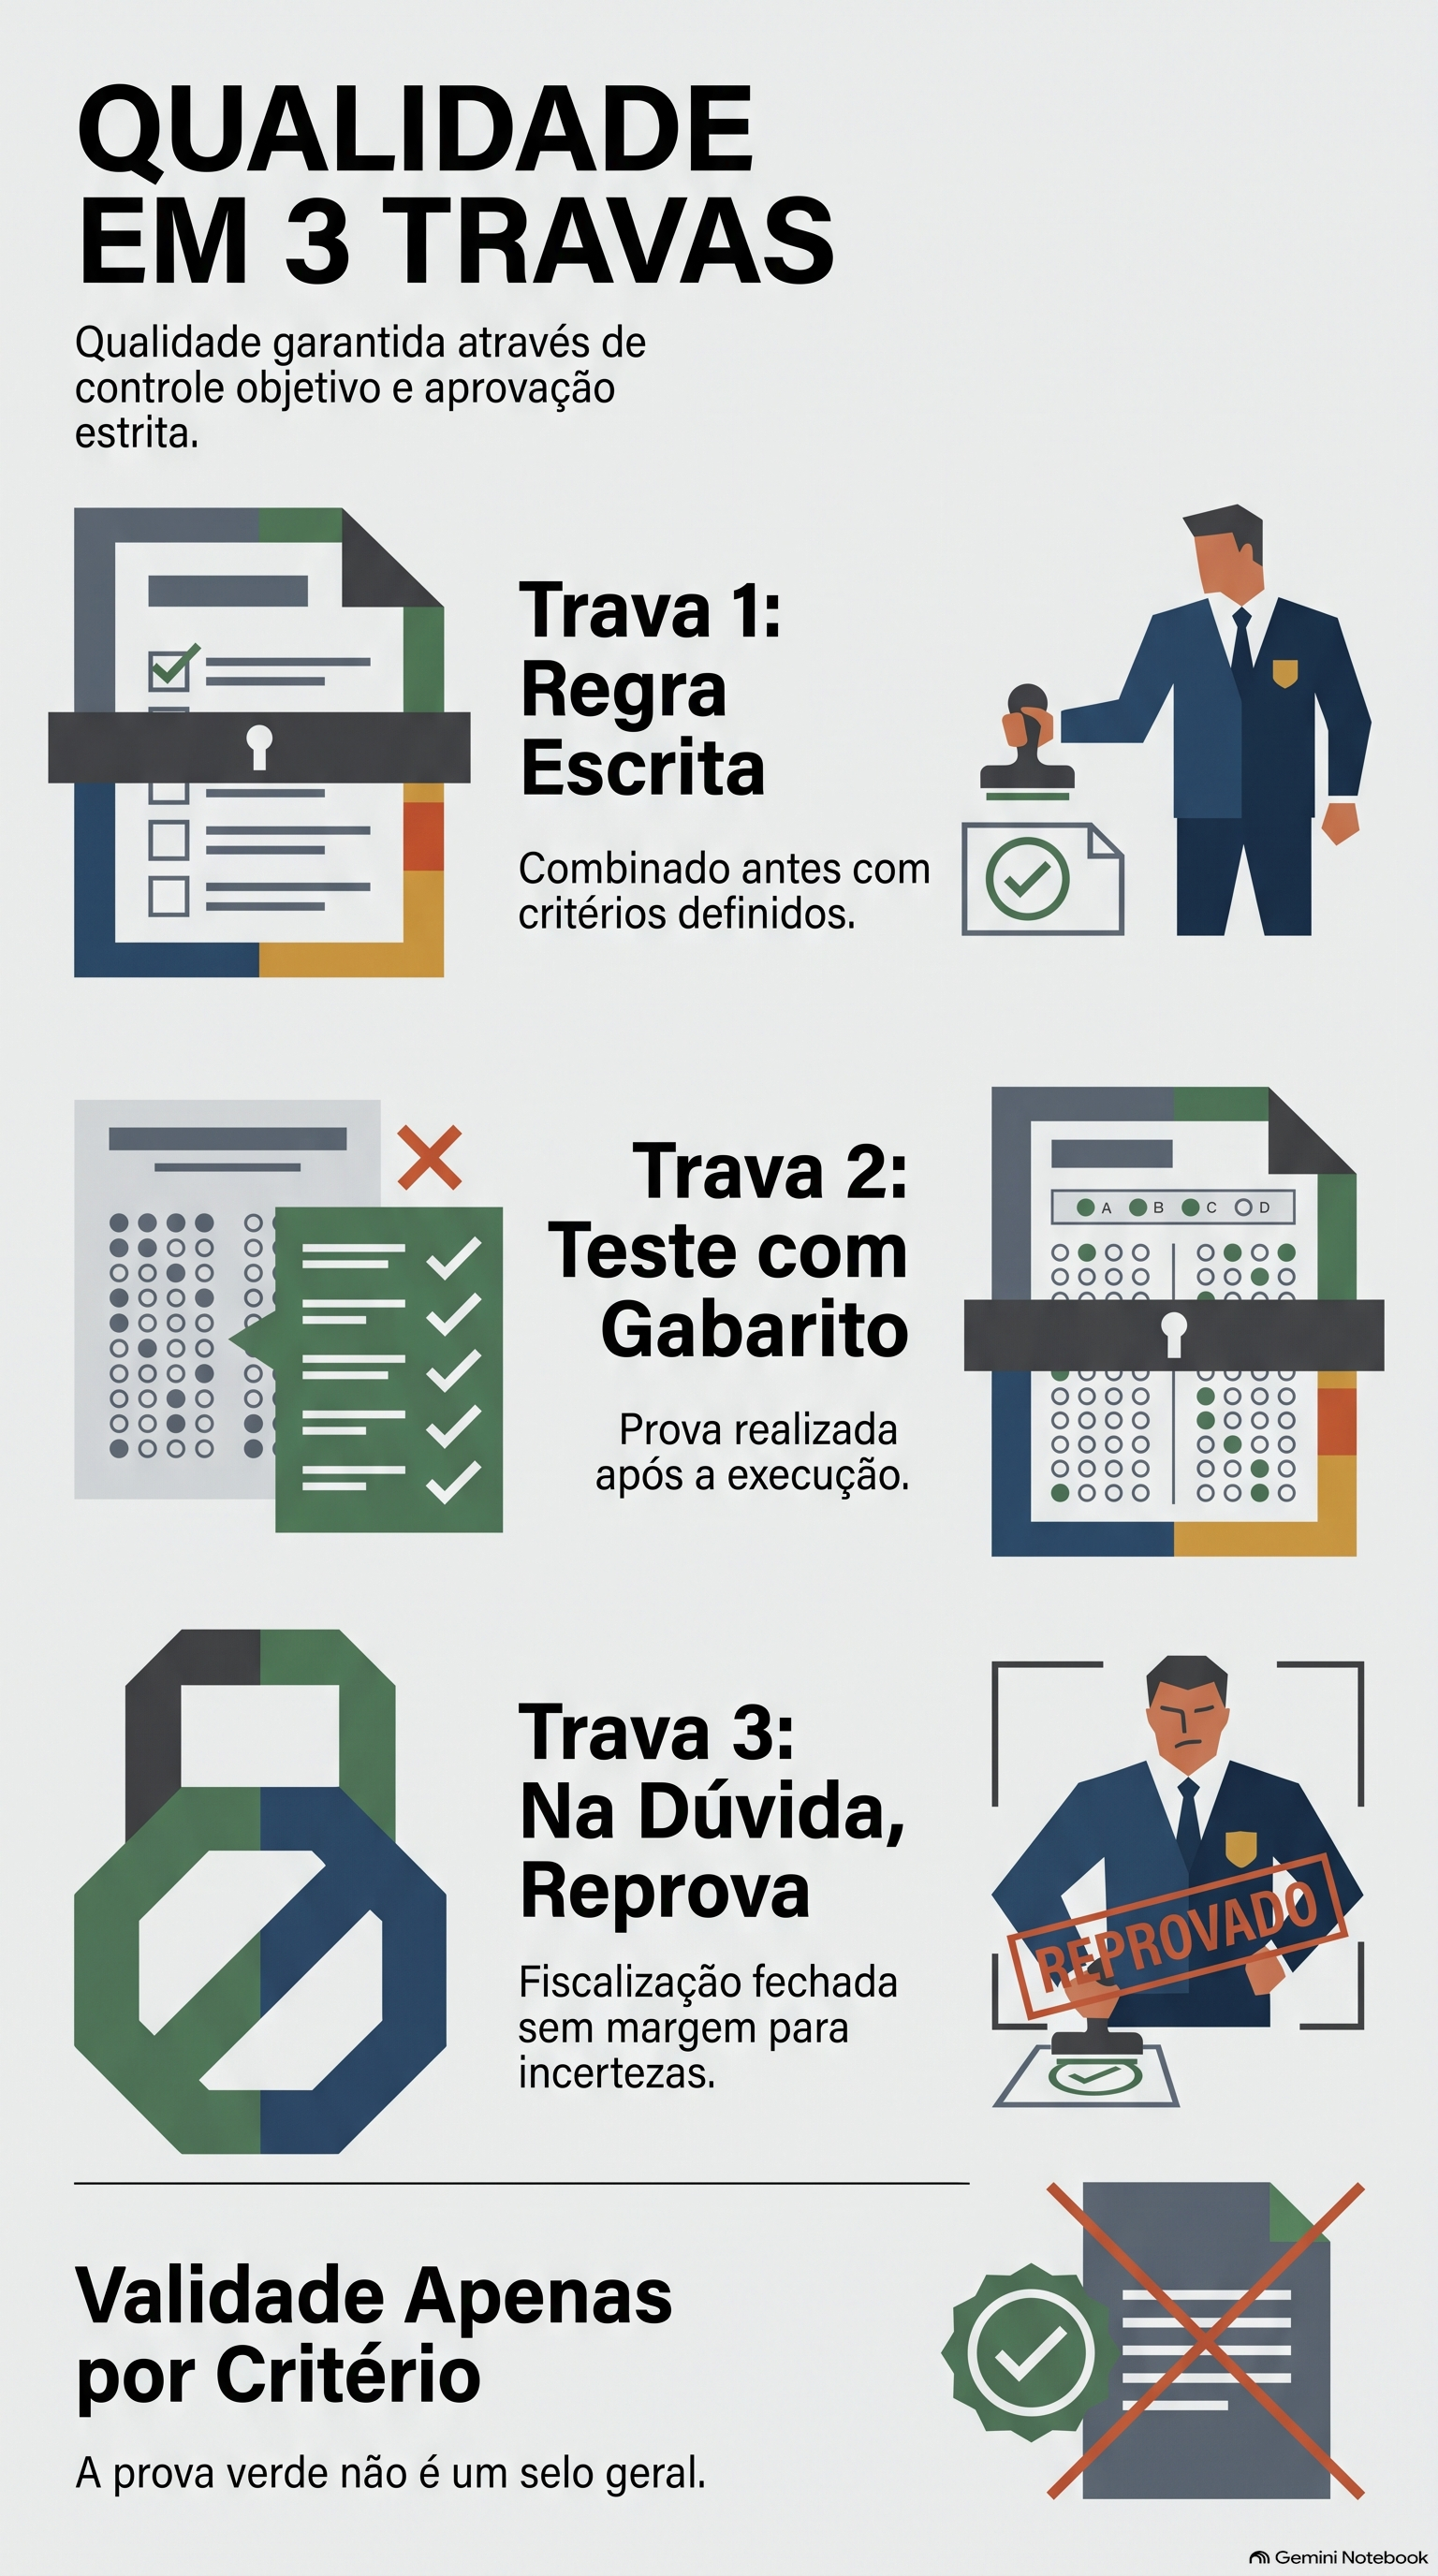
\includegraphics[width=0.96\linewidth,height=0.80\textheight,keepaspectratio]{INF-S05-fiscal-curto.png}
\end{center}

\elemento{INF-S06 — Números e 12 passos}{\metainfo{ID}{INF-S06} \hfill \metainfo{Arquivo}{\pth{INF-S06-numeros-curta.png}} \hfill \metainfo{Capítulo}{mod-15 e mod-22}}

\begin{descricao}
Os números 62 e 94 pertencem ao exemplo da ilustração; não são uma medição corrente desta revisão. A figura apresenta também rastreabilidade (origem, versão, código) e a trilha de 12 passos. Para relatar desempenho, consulte o experimento e seu escopo em vez de reutilizar o número do desenho.
\end{descricao}

\begin{center}
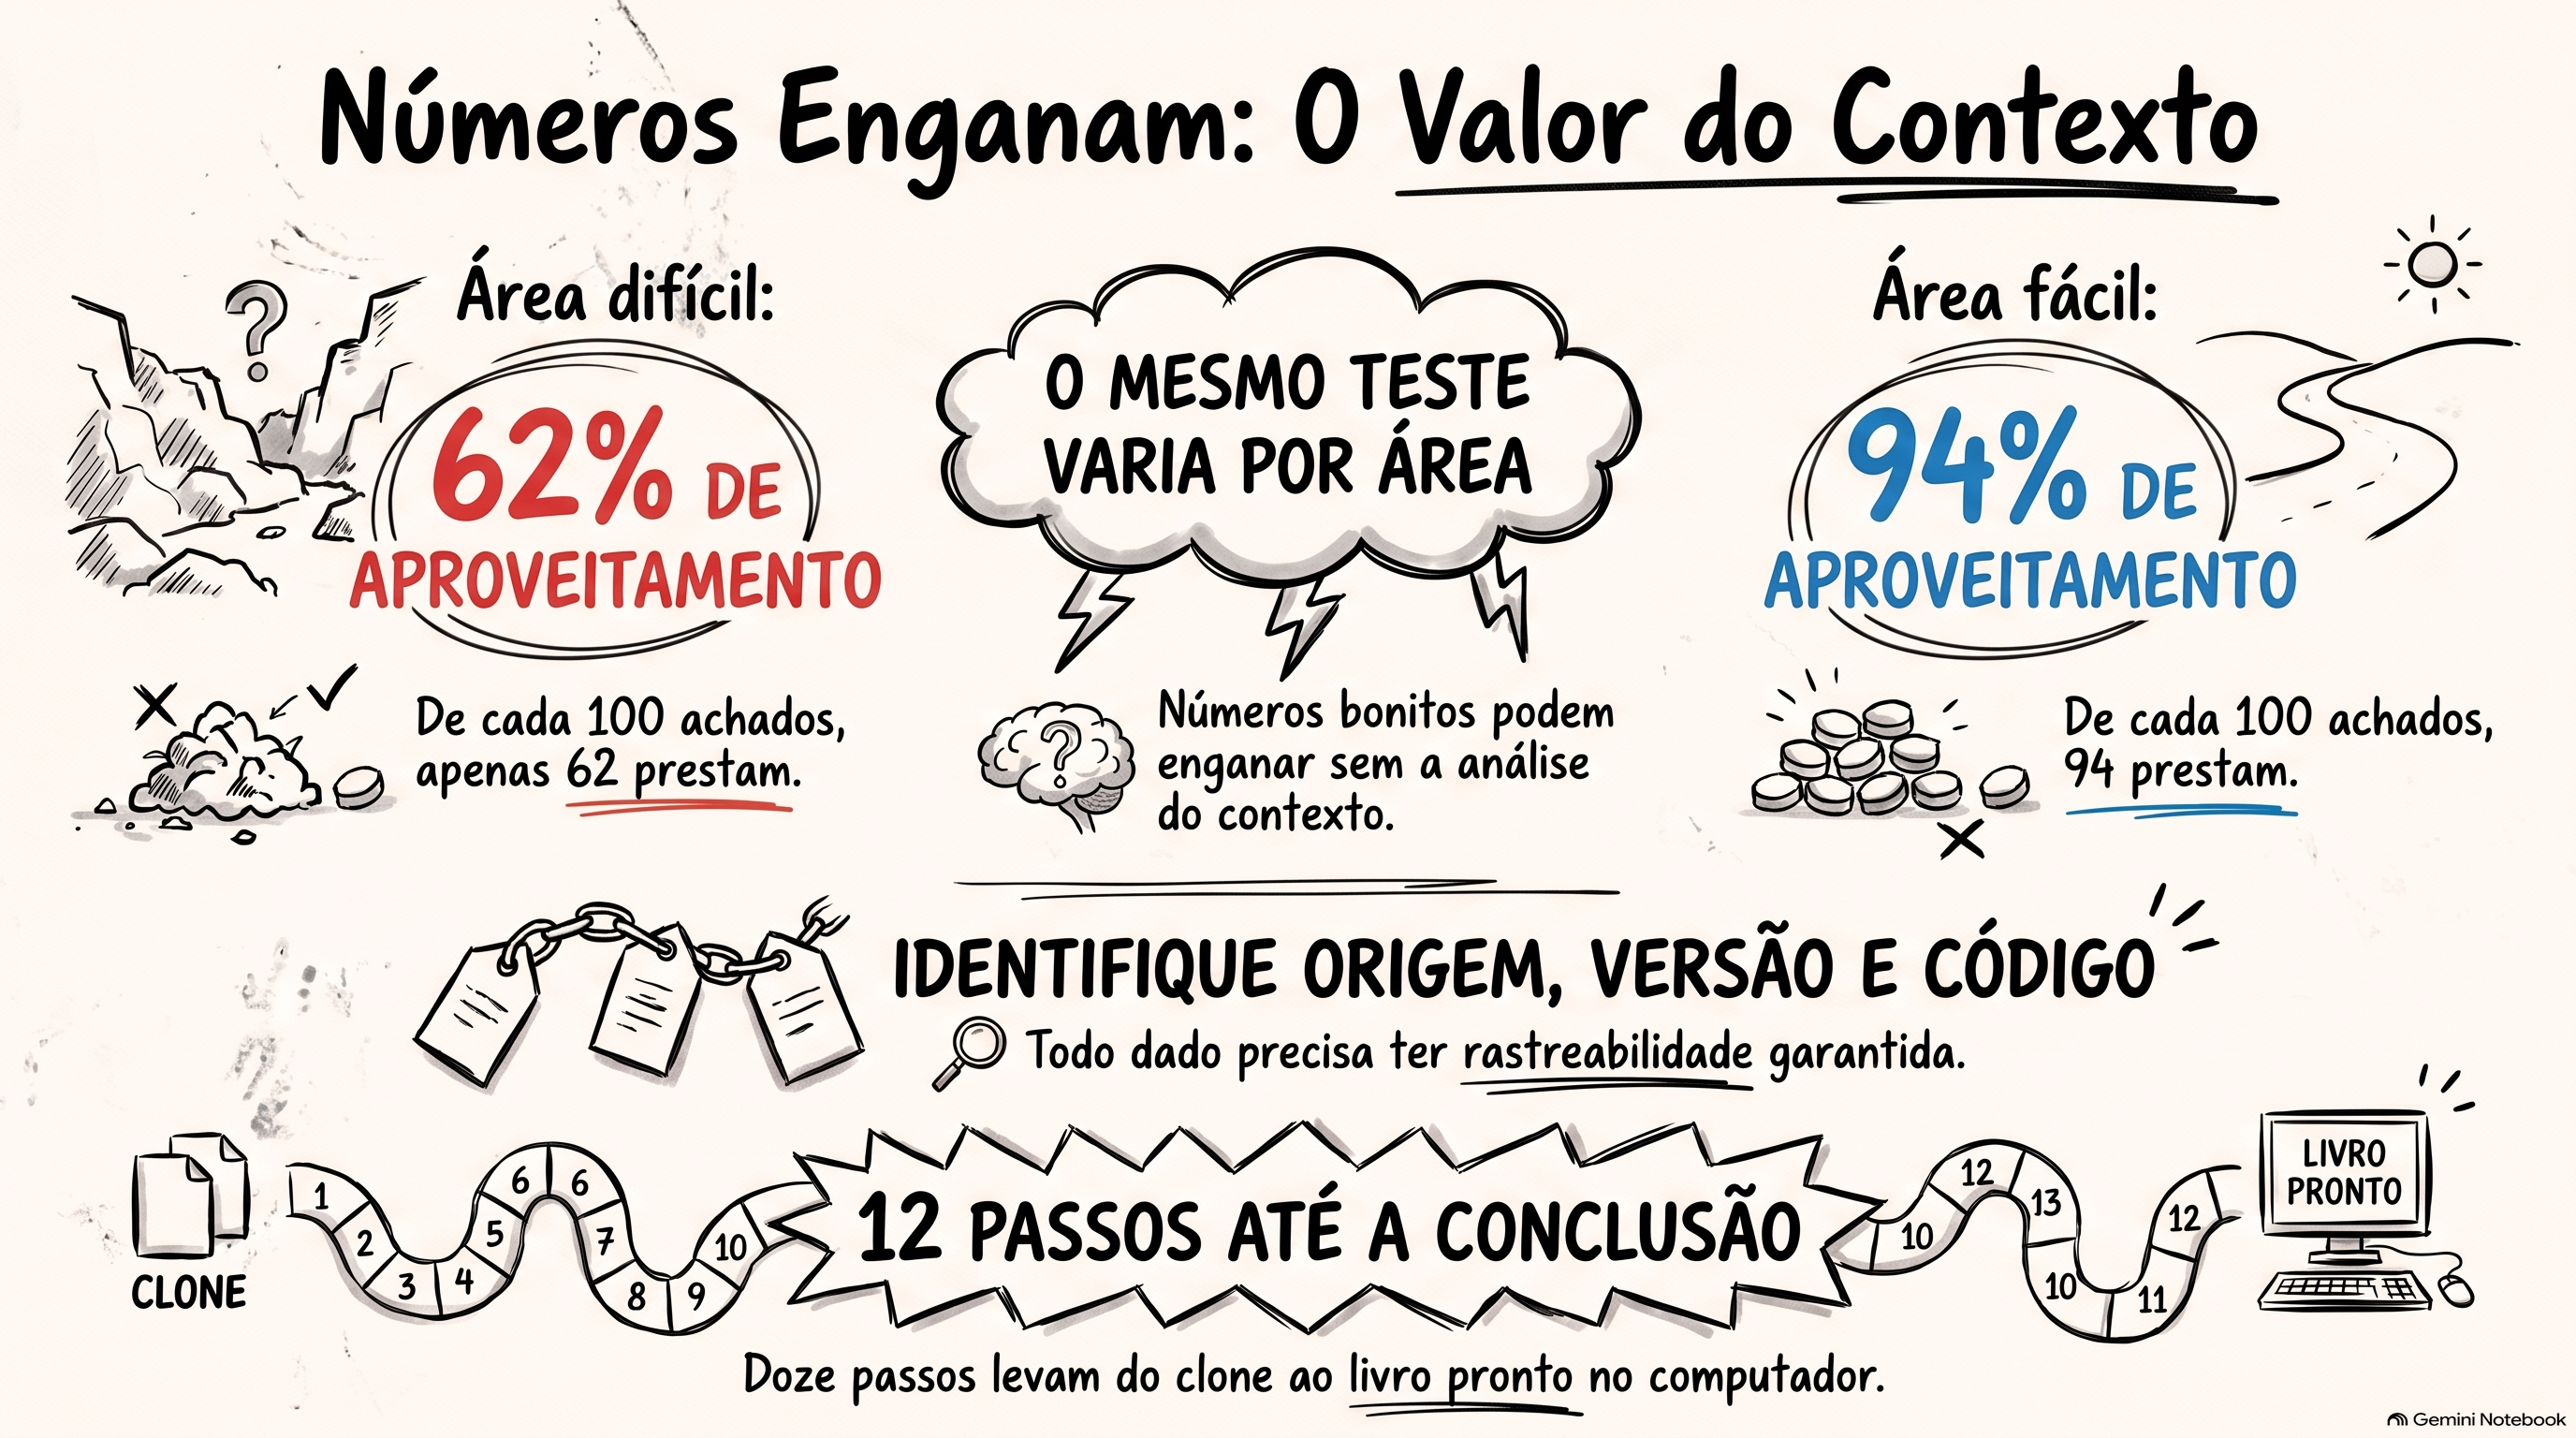
\includegraphics[width=0.96\linewidth,height=0.80\textheight,keepaspectratio]{INF-S06-numeros-curta.png}
\end{center}

\begin{funcao}
Dar ao professor um kit imprimível: 6 A4 para a parede da sala, cada um apontando para o capítulo que o sustenta, sem substituir a leitura.
\end{funcao}

\begin{limite}
Atlas é recurso didático gerado por IA externa (Gemini Notebook) a partir de roteiros curtos do autor, com ortografia do texto principal conferida por leitura visual em 11/10/2026. Números em ícones decorativos podem divergir; em caso de divergência, valem capítulo, arquivo e teste. Revisão humana obrigatória antes de uso em sala.
\end{limite}
\fontecore{livro-core/INF-S01-casa-curta.png}{caderno-419f77cb-PNG-curto-1}
\fontecore{livro-core/INF-S02-ciclo-curto.png}{caderno-419f77cb-PNG-curto-2}
\fontecore{livro-core/INF-S03-passos-curta.png}{caderno-419f77cb-PNG-curto-3}
\fontecore{livro-core/INF-S04-lousa-curta.png}{caderno-419f77cb-PNG-curto-4}
\fontecore{livro-core/INF-S05-fiscal-curto.png}{caderno-419f77cb-PNG-curto-5}
\fontecore{livro-core/INF-S06-numeros-curta.png}{caderno-419f77cb-PNG-curto-6}

\section[Leitura guiada]{Leitura guiada: usar a figura sem promover seu conteúdo a prova}
\begin{descricao}
\textbf{O fenômeno.} Uma ilustração facilita a orientação, mas números e setas podem resumir de modo impreciso um mecanismo ou uma medição histórica.
\end{descricao}
\begin{definicao}
\textbf{Grandezas e definições.} Diferencie figura didática, fonte local e recibo de execução. A quantidade de figuras descreve o atlas; não é contagem de experimentos ou validações.
\end{definicao}
\begin{metodo}
\textbf{Dedução passo a passo.} Escolha uma figura; leia sua legenda; localize o capítulo associado; confira cada número na fonte indicada; marque o estado temporal da informação; revise antes de apresentar.
\end{metodo}
\begin{resultado}
\textbf{Exemplo resolvido.} Ana encontra um número decorativo no infográfico que difere do inventário corrente. Ela utiliza o inventário como referência operacional e explica que a figura é uma representação didática; não apresenta o número decorativo como nova medição.
\end{resultado}
\begin{resultado}
\textbf{Ordem de grandeza e verificação.} O atlas contém seis figuras declaradas. Conte os arquivos e confira legibilidade, correspondência com a legenda e limites de cada uma. Se uma figura falhar, registre o problema individualmente.
\end{resultado}
\begin{aviso}
\textbf{Limite de validade.} A inspeção visual registrada em 11/10 tem o alcance descrito na legenda. Ela não calibra métricas nem confirma eficácia do Core. Este capítulo não transforma imagens geradas por IA em dados experimentais.
\end{aviso}
\begin{resultado}
\textbf{Exercícios.} Relacione uma figura a uma fonte; encontre um número que exige data e escopo; descreva uma simplificação do desenho; escreva uma legenda que conserve esse limite.
\end{resultado}
